\section{Introducción}
\label{sec:aim}

\subsection{Contexto y justificación}
\label{subsec:context}

Las bases de datos relacionales llevan con nostros desde hace más de 40 años.
Como bien dice su nombre, están basadas en el modelo relacional, descrito por
Edgar F. Codd en 1970.

Dos de las características deseables de una base de datos relacional bien
diseñada, son la \emph{normalización} y las \emph{transacciones}. A través de
ellas, la consistencia de los datos mejora, es decir, nos aseguramos de que la
base de datos se mantiene en un estado coherente. 

% Es difícil implementar una base de datos relacional distribuida?
% TODO: Describir el aumento de datos a procesar, y brevemente, NoSQL.
% No hace falta enrollarse, aquí simplemente estamos explicando la situación general.

% TODO: Describir ``data science'''


\subsection{Objetivos}
\label{subsec:objectives}

Los objetivos principales del proyecto son:

\begin{itemize}
    \item Estudiar y conocer el SGBD NoSQL Apache Cassandra.
      \begin{itemize}
      \item Identificar los usos ideales para Apache Cassandra.
      \end{itemize}
    \item Entender el modelo de datos y consultas de Apache Cassandra.
    \item Diseñar un sistema para almacenar estadísticas sobre el tráfico de red
      en Apache Cassandra.
    \item Entender y familiarizarse con el flujo de trabajo del \emph{data scientist}.
      \begin{itemize}
      \item Analizar mediante Python los datos obtenidos de Cassandra, y
        intentar predecir el tráfico de red en el futuro.
      \end{itemize}
\end{itemize}

\subsection{Metodología}
\label{subsec:metodologia}

El proyecto se dividirá en dos partes bien diferenciadas: la primera consistirá
de un estudio de las bases de datos NoSQL, en concreto Apache Cassandra, y una
comparativa en base al modelo relacional.

La segunda, consistirá en emplear lo aprendido en la primera parte para
implementar un sistema que aproveche las aptitudes de Cassandra para el
\emph{big data} y el análisis de datos. A éstos efectos, se utilizará Python y
un variado conjunto de librerías para explorar los datos recogidos,
visualizarlos, y intentar predecir el tráfico de red estimado en un punto
concreto del futuro.

\subsection{Características técnicas}
\label{subsec:planificació}

En la siguiente lista se detallan las tecnologías y herramientas que se
utilizarán durante el proyecto:

\begin{itemize}
    \item \textbf{Documento de la memoria: } \LaTeX
    \item \textbf{SGBD NoSQL: } Apache Cassandra
    \item \textbf{Lenguaje de programación: } Python \textbf{Librerías:} \\
      \begin{itemize}
      \item Pandas
      \item statsmodels
      \item matplotlib
      \item Jupyter Notebook
      \end{itemize}
    \item \textbf{Presentación: } Reveal.js
\end{itemize}


\subsection{Planificación del proyecto}
\label{subsec:planificació}

% \subsubsection{Lista de tareas}
% \label{subsubsec:tasklist}

% \includegraphics[page=4,scale=0.75]{salida.pdf}
% 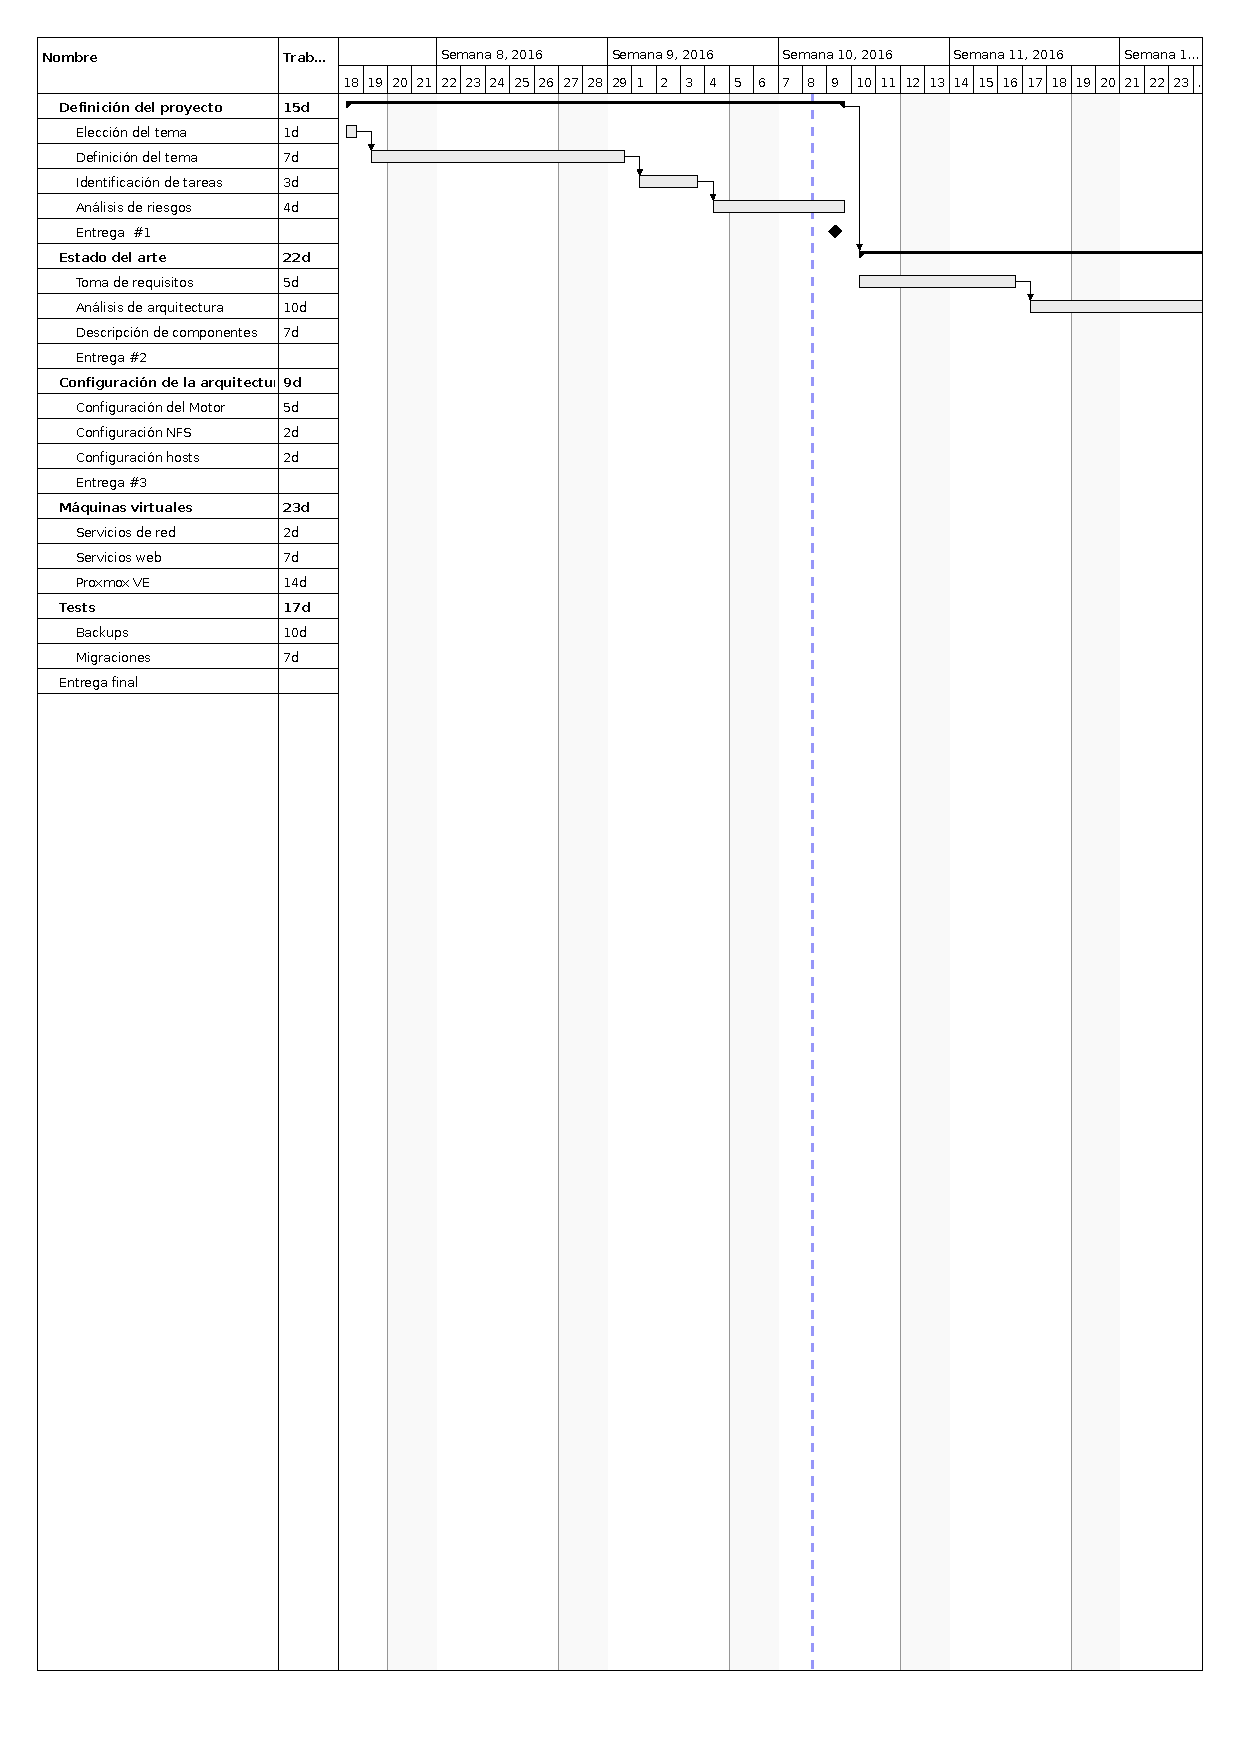
\includepdf[pages={1-3},scale=0.70]{salida.pdf}

\subsubsection{Planificación horaria}
\label{subsubsec:hores}

\subsection{Descripción de los capítulos}
\label{subsec:chaps}

% TODO: Definir la estructura de capítulos y explicarlos brevemente.

\begin{enumerate}
    \item \textbf{Estado del arte: } 
    \item \textbf{Conclusiones: } 
\end{enumerate}
\clearpage
